\documentclass{article}
\usepackage{enumitem}
\usepackage{fancyhdr}
\usepackage{listings}
\usepackage{graphicx}
\usepackage{hyperref}
\usepackage{supertabular}
\usepackage[lastexercise,answerdelayed]{exercise}
\usepackage[table]{xcolor}

% for exercise 
%% Change this for title information 
\newcommand\ExTitle{\ Course Outline and Essential Information}
\author{Mair\'ead Meagher, WIT}

\newcommand\fullExTitle{Functional Programming
\\ \ExTitle \\Semester 2 - '21-'22 }
\newcommand\footerExTitle{\ExTitle -\ Functional Programming }

\pagestyle{fancy}
\fancyhead{} % clear all header fields
\renewcommand{\headrulewidth}{0pt} % no line in header area
\fancyfoot{} % clear all footer fields
\fancyfoot[LE,RO]{\thepage}           % page number in "outer" position of footer line
\fancyfoot[RE,LO]{\footerExTitle} % other info in "inner" position of footer line

%\usepackage[mathrm,colour,cntbysection]{czt}

\begin{document}
\begin{Huge}
	\begin{center}
	\fullExTitle \\
    \vspace{.1cm}
    Mair\'ead Meagher, WIT.
    \end{center}
\end{Huge}
\begin{center}
    \begin{tabular}{|c |  c | }
 
    \hline
    
\includegraphics[width=1.5in]{img/wit.jpg} &          
\includegraphics[width=1.5in]{img/mairead.png} \\ 

   
    %  \rowcolor{red!60}
    %  \textbf{Assignment}& Vet Appl  & Vet Appl  & Prog assign  & Prog assign\\  
    %  \rowcolor{red!60}
    
        & Mair\'ead Meagher  \\  
       & \href{mailto:mmeagher@wit.ie}{mmeagher@wit.ie}, \\

    \hline
    \multicolumn{2}{|c|}{Department of Computing and Mathematics} \\
     \hline

  
    \end{tabular}
\end{center}

\tableofcontents
\pagebreak
\section{Module Name}   
Functional Programming.  \\
This is the year 4, semester 2 running of this module in Waterford Institute of Technnology. 
\section{Lecturer}
Mair\'ead Meagher, \\
Lecturer in Department of Computing and Mathematics, \\
School of Science and Computing, \\
Waterford Institute of Technnology.

\section{How to reach me}
\begin{itemize}
    \item The quickest way to reach me is via Slack (please join the Functional Programming  Slack workspace  
    \href{https://join.slack.com/t/slack-uvg2326/shared_invite/zt-11nr3172s-6T6eSGwcZoUvkRio95rxwA}{here} ).  
    I will be using  this  as the main form of communication for this running of the module. 
    \item You can also reach me via email: \href{mailto:mmeagher@wit.ie}{mmeagher@wit.ie}. 
    \item I am available during work hours from Monday to Friday, 9am to 5pm. You can email me / Slack me outside of these hours and I will reply as soon as I can, 
but always within three days.(If this does not happen, assume your contact has gone into spam etc. and please re-contact me.) When emailing me, please indicate what module you are taking as well as the nature of your query in the 
subject line, and do not forget to use an appropriate greeting and sign off. It’s important to be polite and to treat one another with 
respect; let’s start as we mean to go on.
    \item I will be giving face-to-face weekly lectures(public health advice allowing), but if I need to  meet you via Zoom, the link for these meetings is here: \href{https://wit-ie.zoom.us/j/94189213426}{FP Zoom Link}  (I will usually send this to you on Slack beforehand anyway).
\end{itemize}
\section{Learning Technologies}
We will be using 
\begin{itemize}
    \item \textbf{Moodle} - our learning management system, where you can find links to the notes, and where online exams are curated. The link to this course is \href{https://join.slack.com/t/functprog22/shared_invite/zt-11nr3172s-6T6eSGwcZoUvkRio95rxwA}{here}.  
Each week you will be given a list of activities to have done before the class and a list of activities to have done before the next week. See Figure \ref{fig:todo}
\begin{figure}[h]
    \centering
    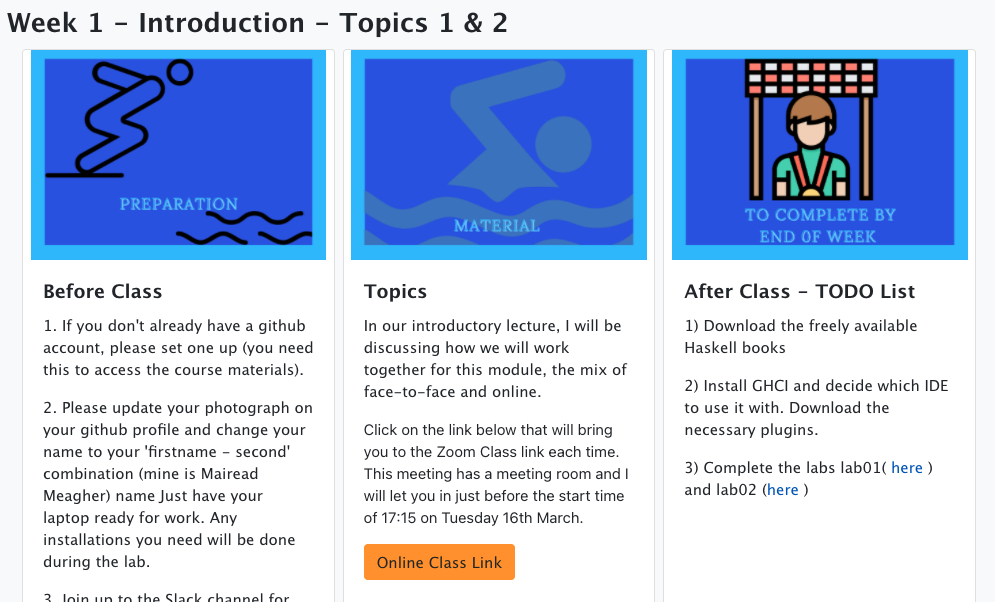
\includegraphics[width=3in]{img/week-todo.png}
    \caption{Example of a weekly activity in Moodle}
    \label{fig:todo}
\end{figure}


    \item \textbf{Zoom} - (link \href{https://wit-ie.zoom.us/j/94189213426}{here} for any meetings we have on Zoom)-  a videoconferencing application that 
    allows for synchronous learning including the use of small group work, or “breakout rooms” - we may  use this from time to time. 

    \item \textbf{tutors} - This static website will hold all the notes, labs and links to videos. There will be a pre-recorded lecture associated with each lecture. See Figure \ref{tutors}.
    This site has the full course published so you can navigate in whatever way suits you.  
\begin{figure}[h]
    \centering
    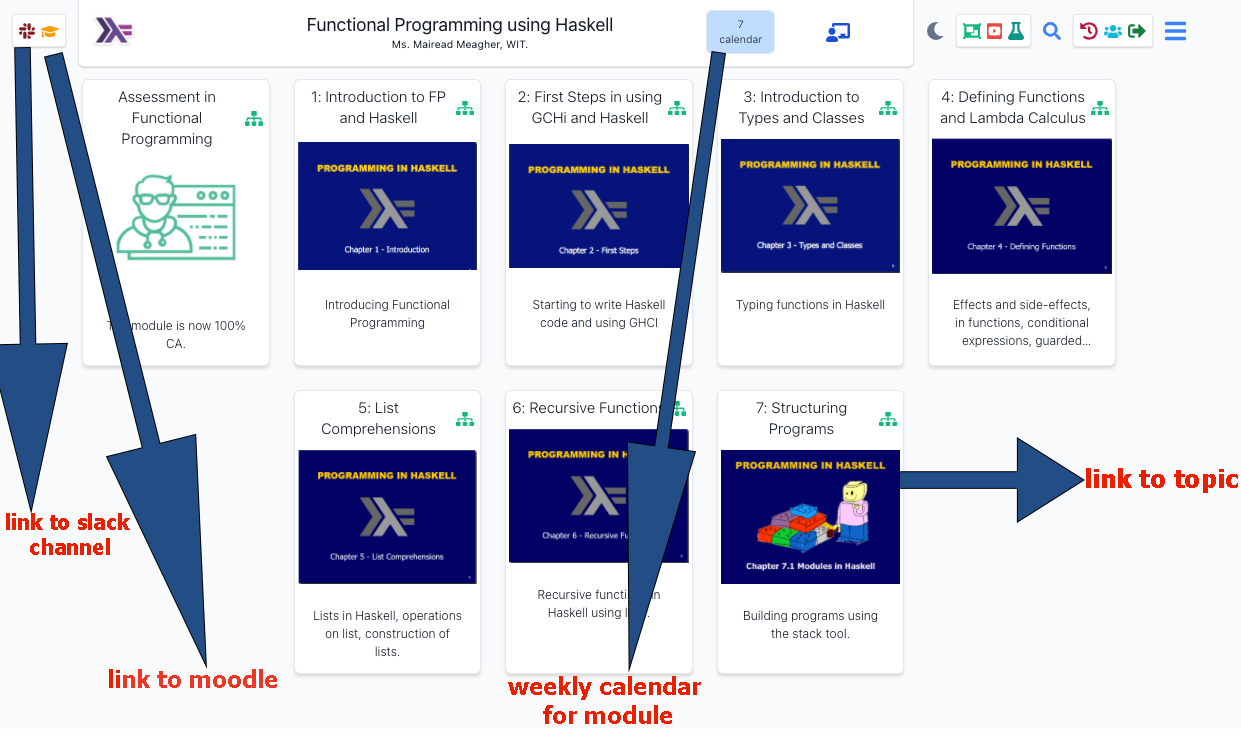
\includegraphics[width=.9\textwidth]{img/tutors.png}
    \caption{Example of tutors website}
    \label{tutors}
\end{figure}
\\
I will also present each lecture  during timetabled class time.

\end{itemize}
\pagebreak

\section{Module objectives /\ Learning outcomes}
On completion of this module students should be able to: 
\begin{enumerate}
    \item  Construct simple and more complex programs in Haskell;
    \item  Construct basic constructs of Haskell;
    \item  Use tools to help build Haskell projects, notably GHCI and Stack;
    \item  Improve the scope of programs by using Haskell libraries;
    \item  Write programs to solve problems in specific domains, e.g. parsing;
    \item  Write Haskell programs that call other languages and vica versa.
\end{enumerate}
\section{Assessment Breakdown} 
\begin{table}
\begin{center}
    \begin{tabular}{|  c | c | c | c| c |}
        \hline
        \rowcolor{green!50}
        GHCI lab test  & lab test Stack & Prog assignment 1 & Prog assignment 2 & Final Exam \\  
    
    \hline
    \rowcolor{green!20!yellow!40}
    5\% & 5\% & 20\% & 20\% & 50\% \\ 
    \rowcolor{red!60}
    Week 3  & Week 7 & Week 9 & Week 12 & Exam Session \\ 
     \hline
     \rowcolor{red!60}
    Test time/date & Test time/date & Handup time/date & Handup time/date & Time/date of exam \\ 
     \hline
     \rowcolor{red!60}
     11:15,Thurs 03/02 & 11:15,Thurs 10/03 & 18:00, Sun 27/03  & 18:00, Sun, 01/05 & tbc \\ 
     \hline
     \rowcolor{blue!40}
     & & Interviews:week 10 &Interviews: Week 13 &\\ 


     \hline
  
    \end{tabular}
    \caption{Assignment Schedule}
    \label{tab:ass-schedule}   
    
\end{center}
\end{table}
The asessment in this module is made up of continuous assessment during the module and a Final Exam at the end of the semester. 
The schedule\footnote{these times are timetable dependant- they may have to change if the timetable changes but they will be during that week} is seen at Table \ref{tab:ass-schedule} - Assignment Schedule. 
\begin{enumerate}

    \item  \textbf{Continuous Assessment} (50\%) broken into 
    \begin{itemize}
        \item In-class lab test - 5\% - starting using GHCI – this is to ensure that all students are competent in using GHCI and writing small Haskell programs. It includes fixing syntax errors, e.g. filling in missing type declarations in simple functions.
        \item In-class lab test - 5\% - using Stack – a simple program using the Stack structure.
        \item  20\% programming assignment 1
        \item  20\% programming assignment 2 
    \end{itemize}
    \item \textbf{Written Final Exam} (50\%) subject to public health advice, this is planned to be a written final exam. 
\end{enumerate}



The CA is rolled out in the above order so that you, the student, can steadily build up marks throughout the semester. 

For all the continuous assessment submitted during the module, you will get your marks back as soon as is possible, but usually within a week. 
If you are wondering why you got a particular mark, \textbf{always} ask me. My marking schemes are very comprehensive and I am happy to go through the breakdowns with you. 
I don't give this comprehensive feedback by default to speed up the return of the marks but am happy to engage about them later. 

For the in-class lab tests, I will give you sample lab tests so that you know the nature of the tests beforehand. 

For the programming assignments, a marking scheme will be published with the specification of the assignment. As always, be sure that you are aware of the marking scheme. 
If there are marks going for a particular part, and you haven't attempted that part, there is nothing I can do. Always make it easy for the examiner to give you marks!

If you wish to seek an extension for an assignment, you must do so in sufficient time (i.e. not on the day of submission, and not 
when the submission date has passed) and must provide a valid reason for seeking the extension. 


\section{Academic Integrity}
The School of Science and Computing  at Waterford Institute of Technology are  committed to maintaining the highest standards of academic integrity. 
Academic misconduct, including, but not limited to, cheating may result in a mark of zero for the assignment as well as disciplinary action.
Additional sanctions may by imposed depending on the case. You are responsible for ensuring that you do not get involved in cheating of any kind. 
 
With regard to programming submissions, an interview is mandatory and is part of your assignment mark (as a multiplier). 
The interview is to ascertain that the work is your own and that you fully understand how it works, in its elemental parts and how it works together. 
 
We  will always encourage you to work in collaboration with your fellow classmates. But please be careful not to cross the line between collaboration and using someone else's work. 
Please do not be tempted to use this route. 
It is too risky and the penalty can affect your academic future. 

\pagebreak
\section{Important note about engagement in the module  and time management}
 Part of active engagement  for any module involves a degree of time management. 
 As part of this module I will be asking you to complete exercises, between class times. In some cases I will be asking you to read material before class. 
 (These tasks will be clearly signalled to you at the time). These will not be graded but, by engaging in these tasks at the time, you will be in a better position to 
 understand the next part of the module. We will approach the module in a step-by-step manner, so opting out at any part will make it more difficult for you to keep up. 
 This is where time management will come in - you need to be careful to ensure that you keep a balance between modules. 
 
 Always ask questions, either in class or in a breakout room. I know that online lectures can be hard to keep engaged in. One way to help to stay engaged is to ask questions if you don't understand what is going on. 
 Remember, when you are asking questions:
 \begin{enumerate}
    \item Just the process of asking a question means that you have learned something. 
    \item If you cannot understand, in most cases, you are not the only one. 
    \item Asking questions means that the pace of the lecture/ labs will suit you better - we will always keep going if there are no questions! 
 \end{enumerate}

 \section{Netiquette and Decorum}
 In all of our asynchronous discussions online, mostly Slack for us,  it is important that we foster a supportive, safe, 
 and engaging learning environment where we can critically discuss, analyse, and reflect on the 
 readings and topics each week. Diverse views are encouraged and welcomed and should be based on evidence. 
 You are free to express your views and ideas as long as your words or action do not demean, intimidate, or intend
  to violate the rights and dignities of others. Hate speech is not acceptable and may result in disciplinary action. 
 Hate speech includes words or actions that threaten or target the safety and liberties of an individual or group.
   
 \subsection{Netiquette}
 The word netiquette is a combination of ’net’ (from internet) and ’etiquette’. It means respecting other users’ views and displaying 
 courtesy when posting your views to online discussion groups (see \href{https://www.bbc.co.uk/webwise/guides/about-netiquette}{BBC})
 \begin{itemize}
    \item Remember that there is a human being on the other end of your communication
    \item Treat that human being with respect
    \item Do not post a message that you would not be willing to communicate in a face to face environment.
    \item Keep it courteous
    \item Be kind and professional:  Online communication comes with a level of anonymity that doesn’t exist when you’re talking to someone face-to-face. 
    Sometimes this leads people to behave rudely when they disagree with one another. Online students probably don’t have the complete anonymity that comes with using a screen name, but you could still fall prey to treating someone poorly because of the distance between screens. Make a point to be kind and respectful in your comments—even if you disagree with someone.
    \item Extend your good nature online: The digital world is an increasingly important part of our lives. We should be our best selves there too. The manners our parents taught us apply everywhere.
    \item Promote healthy discussions: 
    To get the most out of online forums, a useful netiquette guideline is to promote healthy discussion. You can help your online community by posing questions, sharing experiences, providing positive feedback, asking follow-up questions, and referring to information sources. Being a positive contributor is better than being a critic, troll or other negative force.
    \item Ignore inflammatory comments by trolls
    It's generally best to ignore trolls. These are internet users who try to bait other users into a reaction. Trolls might be honest in what they're saying, or they could be sarcastic or deliberately dishonest. You can tell a troll by the inflammatory nature of their statements. They want to stir up negative emotions and responses.
    \item  Respect others as equals:
    Show a little respect and humility online. Think – that idiot who wrote the opinion you completely disagree with is a human being. They have feelings and experiences. They may believe passionately in what they're saying. And they may actually be right.
    Even if you're feeling dismissive or knowledgeable or whatever, inject respect into your writing. That's just being fair to others.
    \item You're here to learn and contribute, not dictate: 
    While we all like to think that our opinion matters, you'll gain more from internet forums by approaching them as a learner.
    When everyone is trying to express their view rather than hearing from others, forums become noisy, crowded with posts, and disjointed. 
    A more polite and effective path is to adopt a listening mode. Read posts carefully, ask questions, and write something only if it offers value to the discussion.
    \item Read first
    Take some time to read through each of the previous discussion post responses before writing your own response. Remember, discussions can move fairly quickly so it’s important to absorb all of the information before crafting your reply. Building upon a classmate’s thought or attempting to add something new to the conversation will show your instructor you’ve been paying attention.
    \item Remember, your words are permanent: Be careful with what you post online. Once it's out there, you may not be able to get it back.
    \item Make your point in a nice way:
    Write in a way to get the kind of reaction you want. A little thoughtfulness, strategy and netiquette can go a long way in online discussions.
    Your first draft of an online post is unlikely to be your best. Are you disagreeing with someone in a flippant way? Have you misinterpreted what they really meant? Will you put people off with the tone of your text.
    \item Pause before you post:
    It's worth taking a moment to reflect before hitting the send button.
    When you're using a computer, you're normally clicking, and scrolling and typing all over the place. Most things are done quickly. But one time when it's important to slow down is when you're about to post something online for all the world to see. Pause and reflect for a second. Are you truly comfortable with what you're sending?
    \item Respect the opinion of your classmates: 
    If you feel the need to disagree, do so respectfully and acknowledge the valid points in your classmate's argument. If you reply to a question from a classmate, make sure your answer is accurate!
    \item Forgive and Forget
    If you’re offended by something another student says online, keep in mind that you may have misunderstood their intentions. Give them the benefit of the doubt.
    \item Please get dressed for video calls!
     You may be expected to turn your camera on during video calls. Don't wear pjamas, don’t get dressed from the waist up, dress like you would if you were going to a 
     class on campus.
 \end{itemize}
\end{document}